% @TODO Change this
\chapter{Background}
\label{chapter2}

The two key concepts we will introduce in this dissertation are the Contour Tree and Persistent Homology. In order to be able to do this we have to first take a step back and walk the reader through a range of other mathematical disciplines. The preliminaries include Point Set Topology, Differential Topology and Algebraic Topology. We will opt for introducing these fields with a more practical and computational flavour and provide the reader with both the necessary formalism and intuition behind the main definitions and results we will use in the following chapters.

\section{Point Set Topology}

The first branch of Topology we shall encounter is Point Set Topology. It forms the underlying framework on top of which mathematicians build the concepts of continuous spaces and functions. As with many other mathematical disciplines topology is the study of sets that posses mathematical structure. Through point set topology we can define the mathematical structure known as the topology of a set. The topology of a set aims make rigorous the notion of whether two elements of a set are "close" or "near" each other. Elements of a set which are close or near to one another are said to be a part of an open set. We can use the topology of a set to manipulate open sets by combining them to obtain new open sets. In this chapter we will borrow our definitions from one of the standard introductory topology textbooks \cite{intro-topo}.

\begin{defn} Let $X$ be a set and $\tau$ be a set of subsets of $X$. The set $\tau$ is a topology on $X$ when the following holds:  \end{defn}

\begin{itemize}
    \item $X \text{ and } \emptyset \in \tau$.
    \item If $U \text{ and } V \in \tau$ then $U \cap V \in \tau$.
    \item If $\{U_\lambda\}_{\lambda \in \Lambda}$ is a family of subsets of $X$, where $U_\lambda \in \tau$ for all $\lambda \in \Lambda$, then
        $\bigcup_{\lambda \in \Lambda}{U_\lambda} \in \tau$.
\end{itemize}

We will call the elements of $X$ points and the elements of $\tau$ open sets or simply open. An open set is an open neighbourhood of a point when the point is in the open set. We must stress that the topology we endow on a set is by no means unique. For example if $X$ is any set then one topology may be $\{\emptyset, X\}$ and another may consist of all subsets of $X$.

Let us now introduce the topology we are going to use on $\mathbb{R}^n$. It is called the standard topology and it is based on the standard definition of distance between points in Euclidean space. Let $x = (x_1, x_2, ..., x_n)$ be a point in $\mathbb{R}^n$. Then we can define the open ball around $x$ of radius $\epsilon$ as $B_\epsilon(x) = \{y \in \mathbb{R}^n: d(x, y) < \epsilon\}$ where we define the distance function as $d(x, y) = \sqrt{\sum_{i=1}^n{(x_i - y_i)^2}}$. The standard topology on $\mathbb{R}^n$ consists of the open balls around all points of all possible radii and their finite intersections and arbitrary unions.

% But how is it possible to update this? How fast is it? * What do you mean by this? *

The next thing we would like to do is to define a special class of functions that preserve the properties of topological spaces. Those are continuous functions.

\begin{defn} A function $f : X \to Y$ is said to be continuous when the preimage of an open set in $Y$ is an open set in $X$. \end{defn}

In formal notation if $U \in Y$ is open in $Y$ then $f^{-1}(U)$ is open in $X$. This definition captures the intuitive understanding we have of continuity from calculus - if we "slightly adjust" the output of a function in $Y$ then there should be only a "slight change" in input in $X$. The "slight change" is formalised by considering all points in a single open set, as we can think of them as being "near".

% @TODO Add quote
If $f$ is a bijection and $f^{-1}$ is also continuous we will call $f$ a homeomorphism. Homeomorphisms play a special role in topology. Two topological spaces are homeomorphic when there exists a homeomorphism between then. As continuous functions preserve open sets it follows that the two spaces are topologically identical. This is the reason why topologists are mostly interested in classifying and analysing spaces up to homeomorphism. We will call a property of a space that is preserved under homeomorphisms a topological invariant.

%Homeomorphism is the appropriate equivalence relation for topological spaces [].

Now let us introduce our first topological invariant - path connectedness. It captures the idea of a topological space where there is a path between any two of its points.

\begin{defn} Let $X$ be a topological space and let $x, y \in X$ be any two points. A path between $x$ and $y$ in $X$ is a continuous function $f: [0, 1] \to X$ such that $f(0) = x$ and $f(1) = y$.  \end{defn}

% @TODO Add this
Using this definition we can define a path-connected topological space as follows.

\begin{defn} A topological space $X$ is said to be path-connected if there exists a path between any two points $x, y \in X$  \end{defn}

This deceptively simple looking definition actually describes one of the methodologies for analysing topological spaces. Through defining auxiliary some auxiliary structure. In the case of path-connectedness we have employed a two parameter family of utility functions to "measure" a global property of the topological space - whether it is path connected or not. The two parameter family is the collection of all paths between all pairs of points.

An important property of path-connectedness is that the continuous image of a path-connected topological space is also path-connected. Properties like this are crucial in the task of differentiating between topological spaces. If for example one space is path-connected and another one is not there there cannot exists a homeomorphism between them. Consequently they are not homeomorphic and therefore topologically different.

We will now introdue two different way in which you can obtain new topologies from already known topologies. The first way is through the subspace topology. A subspace of a topological space $X$ is any subset of points in $X$.

\begin{defn} Let $A \subseteq X$ be a suspace of $X$. The we define the open sets for a topology on $A$ as the intersection of the open sets in $X$ with $A$. \end{defn}

This means that a set $U \subseteq A$ is open in $A$ exactly when $U = U' \cap A$ where $U'$ is open in $X$. This powerful result allows us to obtain a topology through taking all possible intersections of the open sets in $X$ with $A$. For example let $X = \mathbb{R}$ and $A = [0, 1]$. The set $[0, 1/2) = (-1/2, 1/2) \cap [0, 1]$ is open in $A$ because $(-1/2, 1/2)$ is open in $X$, however the resulting set of the intersection
$[0, 1/2)$ is not open in $X$ (only in $A$).

The second way of obtaining new topologies is via the quotient topology. To understand it we must first define a quotient space. An equivalence relation $\sim$ defined on a topological space $X$ partitions all points in $X$ into equivalence classes. The equivalence class of a point $x \in X$ is the set $[x] = \{y \in X: x \sim y\}$. The set of all equivalence classes is called the quotient of $X$ by $\sim$ and denoted as $X / \sim$. Let also $\pi: X \to X/ \sim$ be the map that takes a point $x$ of $X$ to its equivalence class in $X / \sim$.

\begin{defn} Let $X$ be a topological space and $\sim$ be an equivalen relation defined on $X$. The quotient topology of $X / \sim$ is formed by the sets $U \subseteq X / \sim$ such that $\pi^{-1}(U)$ is open in $X$. \end{defn}

By this definition the function $\pi$ is continuous. We can use this fact to infer that if a topological space $X$ is path-connected then $X / \sim$ is path connected for any equivalence relation $\sim$ because there exists a continuous function $\pi : X \to X / \sim$. An important example is when we take quotients of subsets of topological spaces. Let $A \subseteq X$ and let we can define an equivalence relation as $x \sim y$ whenever both $x, y \in A$. We will call the resulting quotient space $X / A$. The geometrical interpretation of $X / A$ is that all points in $A$ are contracted to a single point and all points in $X$ are left unchanged. As a direct example of this consider the closed disk $D = \{x^2 + y^2 \le 1\}$ and its subset the circle $S^1 = \{x^2 + y^2 = 1\}$.
Then $D / S^1$ is homeomorphic to the three dimensional sphere $S^2 = \{x^2 + y^2 + z^2 = 1\}$. To see why this is true imagine embedding $D$ in the $xy$ plane of a three dimensional space. Now imagine contracting all points along $S^1$ to a single point above the $xy$ plane. The resulting object resembles $S^2$ but with a cusp.

Now we will present our final definition. That of a topological manifold - a mathematical generalisation of a surface.

\begin{defn} A $d-manifold$ is topological space where every point has an open neighbourhood that is homeomorphic to $\mathbb{R}^d$.  \end{defn}

% @TODO Redo last sentence.
Examples of 0-dimensional manifolds are points. Examples of one dimensional manifolds are lines, circles, graphs and curves. Examples for 2-dimensional manifolds are the surfaces we are familiar with from geometry such as the sphere, the torus and so on. In this dissertation we will exclusively be using manifold of dimension up to two. * This is because we are most interested in the visualisation aspect of computational topology and hence would like to limit ourselves to modelling spacial phenomena of up to three dimensions. *

% *Manifolds are the playground where topology meets geometry.*

It is often hard to analyse the topology of a space by just considering its open sets. * In practice it is even computationally infeasible due to the shear number of ways we can combine open sets. * This is why in the following two chapters we will employ additional tools from other fields of mathematics to aid in our analysis of the topology of a space. Two such tools are differentiable function over differentiable spaces and combinatorial approximations of topological spaces.


%Contractable Space.

%Path Connected Space.

%Homotopy.

%All of the low level stuff.

%Manifolds.

%Submanifold.

%Genus of a manifold.


%It is often hard to analyse a space just using it's topology.

%This is why we will use additional tools to investigate the topology of a space.

%Two such tools are differentiable function and decomposition into a simplical complex.

\section{Differential Topology}

Differential topology is the study of differentiable functions defined on differentiable manifolds. One of the leading fields of differential topology is that of Morse Theory \cite{morse-theory-book, morse-theory-book-milnor}. Morse theory is the study of the relation between spaces and functions defined on them. One of the main goals is to determine the shape of a shape by analysing the class of functions that can be defined on it. For example using methods from differential topology we can show that the real line and the circle are different topologically. * See Appendix for example.*

One way we can study smooth manifolds via differentiable functions is by analysing the critical points of the functions. This however is an enormous task in its own right. This is why we will restrict ourself to a special class of differentiable functions called Morse functions.

\begin{defn} A function $f: M \to \mathbb{R}^n$ is a Morse Function if $f$ is smooth and at critical points the Hessian (matrix of second partial derivatives) is full rank.   \end{defn}

For practical considerations we will restrict our attention even further and consider Morse functions whose codomain is $\mathbb{R}$. One way we can use a Morse function defined on a manifold is to decompose the manifold into a family of nested subsets. We can then analyse the subsets to obtain some global topological information. Examples of such familiest of subsets are level sets, sublevel sets and super level sets.

\begin{defn} A level set at a value $h$ of a Morse function $f: M \to \mathbb{R}$ is the set $f^{-1}(\{h\}) = \{x \in M: f(x) = h \}$   \end{defn}

Sublevel sets are defined in terms of the preimage of $f$ of intervals of the form $[-\infty, a]$. The sublevel set at $a$ is defined as $f^{-1}([-\infty, a]) = \{x \in M: f(x) \in [-\infty, a] \}$. Superlevel sets are defined analogously in terms of intervals of the form $[a, \infty]$.
% @TODO Include this somewhere else?
% We will call the path-connected components of a level set contours.

% @TODO Explain Critical Points and Critical Value.

Morse functions ensures the following properties which we will make use of in the future:

\begin{itemize}
    \item None of the critical points of a Morse function are degenerate.
    \item Changes in the topology of (sub/super)level sets only happen at critical values. We will call those points critical points.
    \item A Morse function defined on a closed surface has a finite number of critical points.
\end{itemize}

As we saw Morse functions allow us to decompose a manifold into its level sets. We can explore how the connectivity of the level sets changes as we vary the parameter using the abstraction of Reeb Graph.

\subsection{Reeb Graph}

% @TODO Define the quotient topology. Also I'm not sure if you definition of reeb graph is correct!


The Reeb Graph is a tool that encapsulates the evolution of the topology of level sets of a continuous function. When the function is Morse, an edge in the Reeb Graph corresponds to a sequence of contours in the level sets whose topology does not change. The vertices correspond to critical points where the topology of those components does changes. Example of a topological change is when connected components in the level sets appear or dissapear or when two connected components split or merge. * Morse theory ensures that critical points occur at distinct values of the parameter and are isolated. This removes any ambiguities that may arise in the construction of the graph. Furthermore that fact that their number is finite on a close surface and the fact that they only happen at critical values make this computation tractable. *

\begin{defn}
Given a topological space $X$ and a continuous function $f: X \to \mathbb{R}$ we can define an equivalence relation $\sim$ such that two points $x, y$ in $X$ are equivalent when there exists a path between them in a level set $f^{-1}(\{h\})$ for some $h \in \mathbb{R}$. The Reeb Graph is the quotient space $X \big/ \sim$ together with the quotient topology.
\end{defn}

Intuitively we can think of the Reeb Graph of the space where connected components of $X$ are contracted to a single point. We can turn the resulting topological graph into a combinatorial structures by recording all the vertices and edges between them.

*SHOW LOTS OF PICTURES*

The reason we have define reeb graphs is because a contour tree is a special case of the reeb graph. We will come back to this in the begining of the next chapter. Before we move on we must take a look at certain tools from Algebraic Topology that allows us to translate the continuous mathematical results we have obtained so far into the realm of finite combinatorial structures that would allow us to perform actual computation.

\section{Algebraic Topology}

% @TODO Incorrect English in last sentece
Algebraic Topology is a branch of topology that uses tools from the field of abstract algebra to study topological spaces. The primary goal is to derive algebraic structures such as groups, rings and vector spaces from topological spaces that remain invariant under continuous mappings. Modern Algebraic Topology has its roots in combinatorially defined topological spaces \cite{comb-alg-topo}. Unlike Point Set Topology and Differential Topology this allows us to obtain exact algorithm for computing the algebraic invariant we are interested in. To make matters clearer firstly we will introduce one of the most basic combinatorial topological space - Simplicial Comlexes and then we will introduce one of the earliest discovered algebraic invariants - the Euler Characteristic. We will continue our discussion on Algebraic Topology in Chapter Five where we will see how the concept of the Euler Characteristic can be generalised to the one a field of Algebraic Topology called Homology.

\subsection{Simplicial Complexes}

Simplical Complexes are the one of the first combinatorially flavoured topological spaces one encounters in Algebraic Topology. A simplicial complex is a set that consists of points, line segments, triangles and their higher dimensional analogues all "glued together" in a single structure. In order to understand simplicial complexes we must first understand what their basic building blocks are \cite{comp-topo}.

\begin{defn} Let $\{v_0, ..., v_k\}$ be points in $\mathbb{R}^d$. The convex combination of the points is the sum $\sum_{i=0}^k{\lambda_ix_i}$ where $\lambda_i \ge 0$ and $\sum_{i=0}^n{\lambda_i} = 1$.  \end{defn}

If we decide to take the subset of $\mathbb{R}^d$ covered by all possible convex combination we obtain the convex hull of the points.

\begin{defn} Let $\{v_0, ..., v_k\}$ be points in $\mathbb{R}^{k+1}$. We will call the convex combination of those points the $k-simplex$ defined by the points.  \end{defn}

* Show Examples *

\begin{figure}[h]%
    \centering
    \subfloat[Vertex]{{
\includegraphics[scale=0.025]{./images/simplex/vertex.eps}}}%
    \subfloat[Edge]{{
\includegraphics[scale=0.025]{./images/simplex/edge.eps}}}%
    \subfloat[Triangle]{{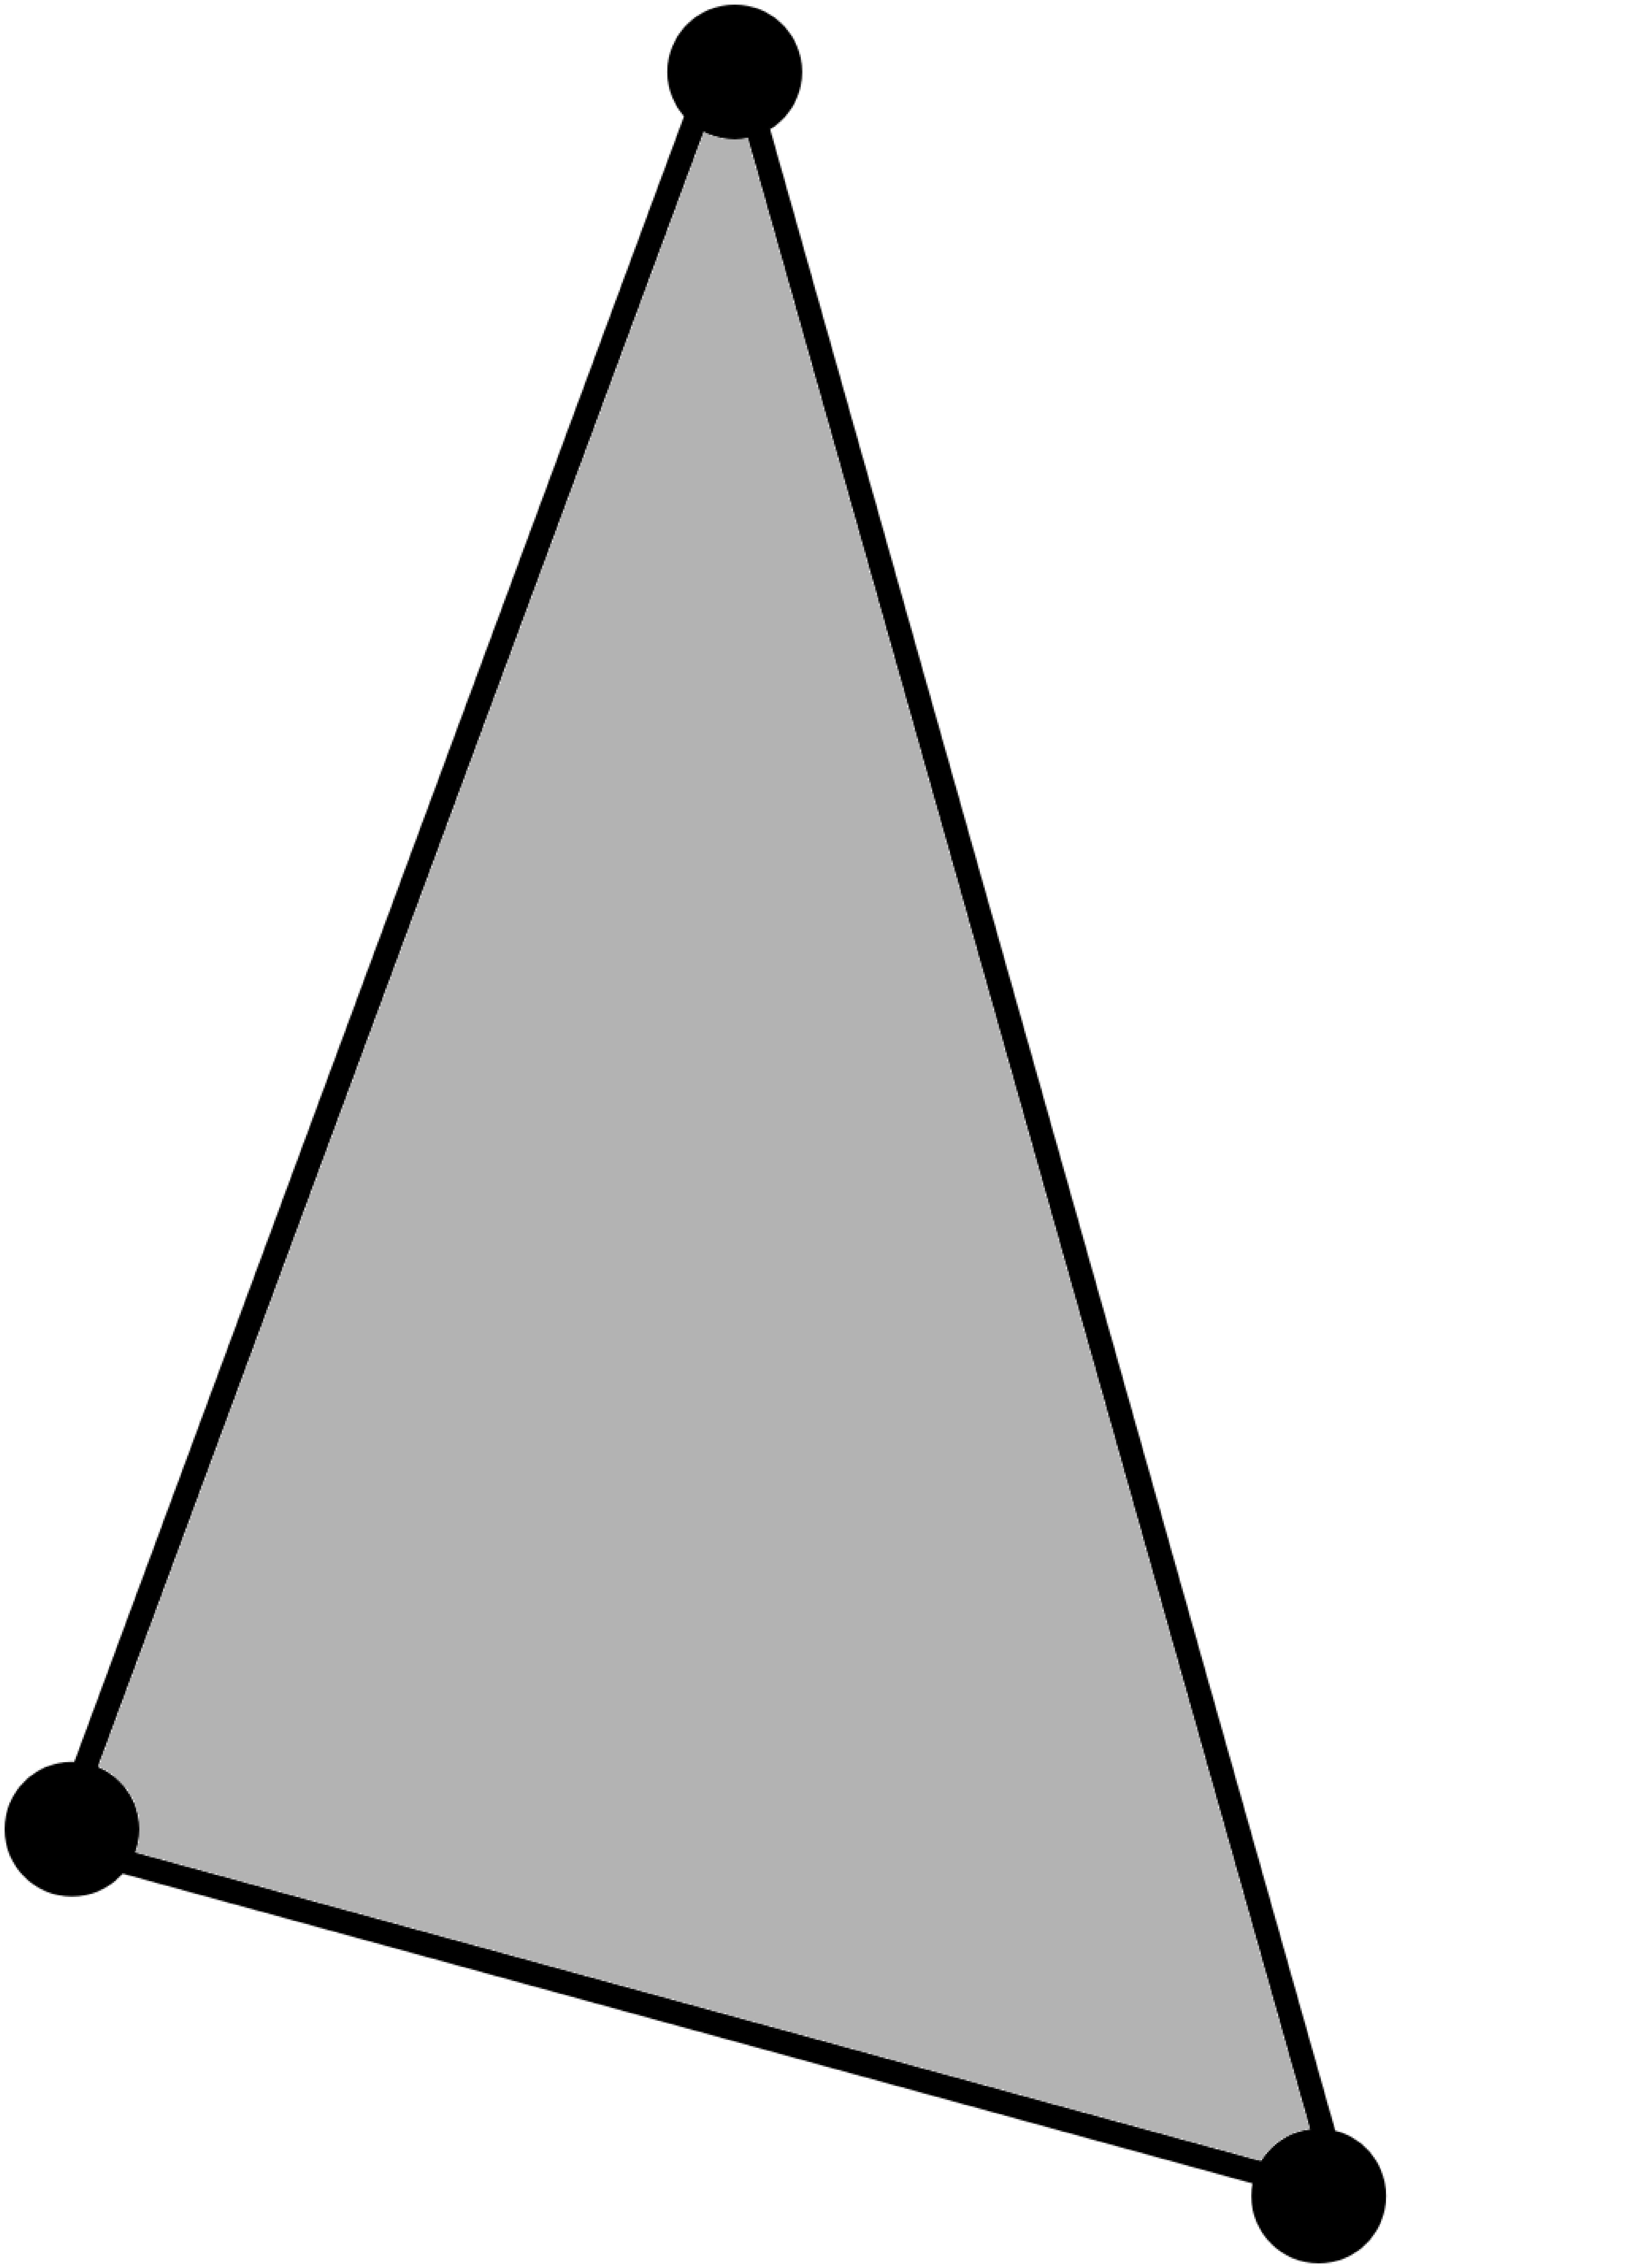
\includegraphics[scale=0.025]{./images/simplex/triangle.eps}}}%
    \subfloat[Tetrahedron]{{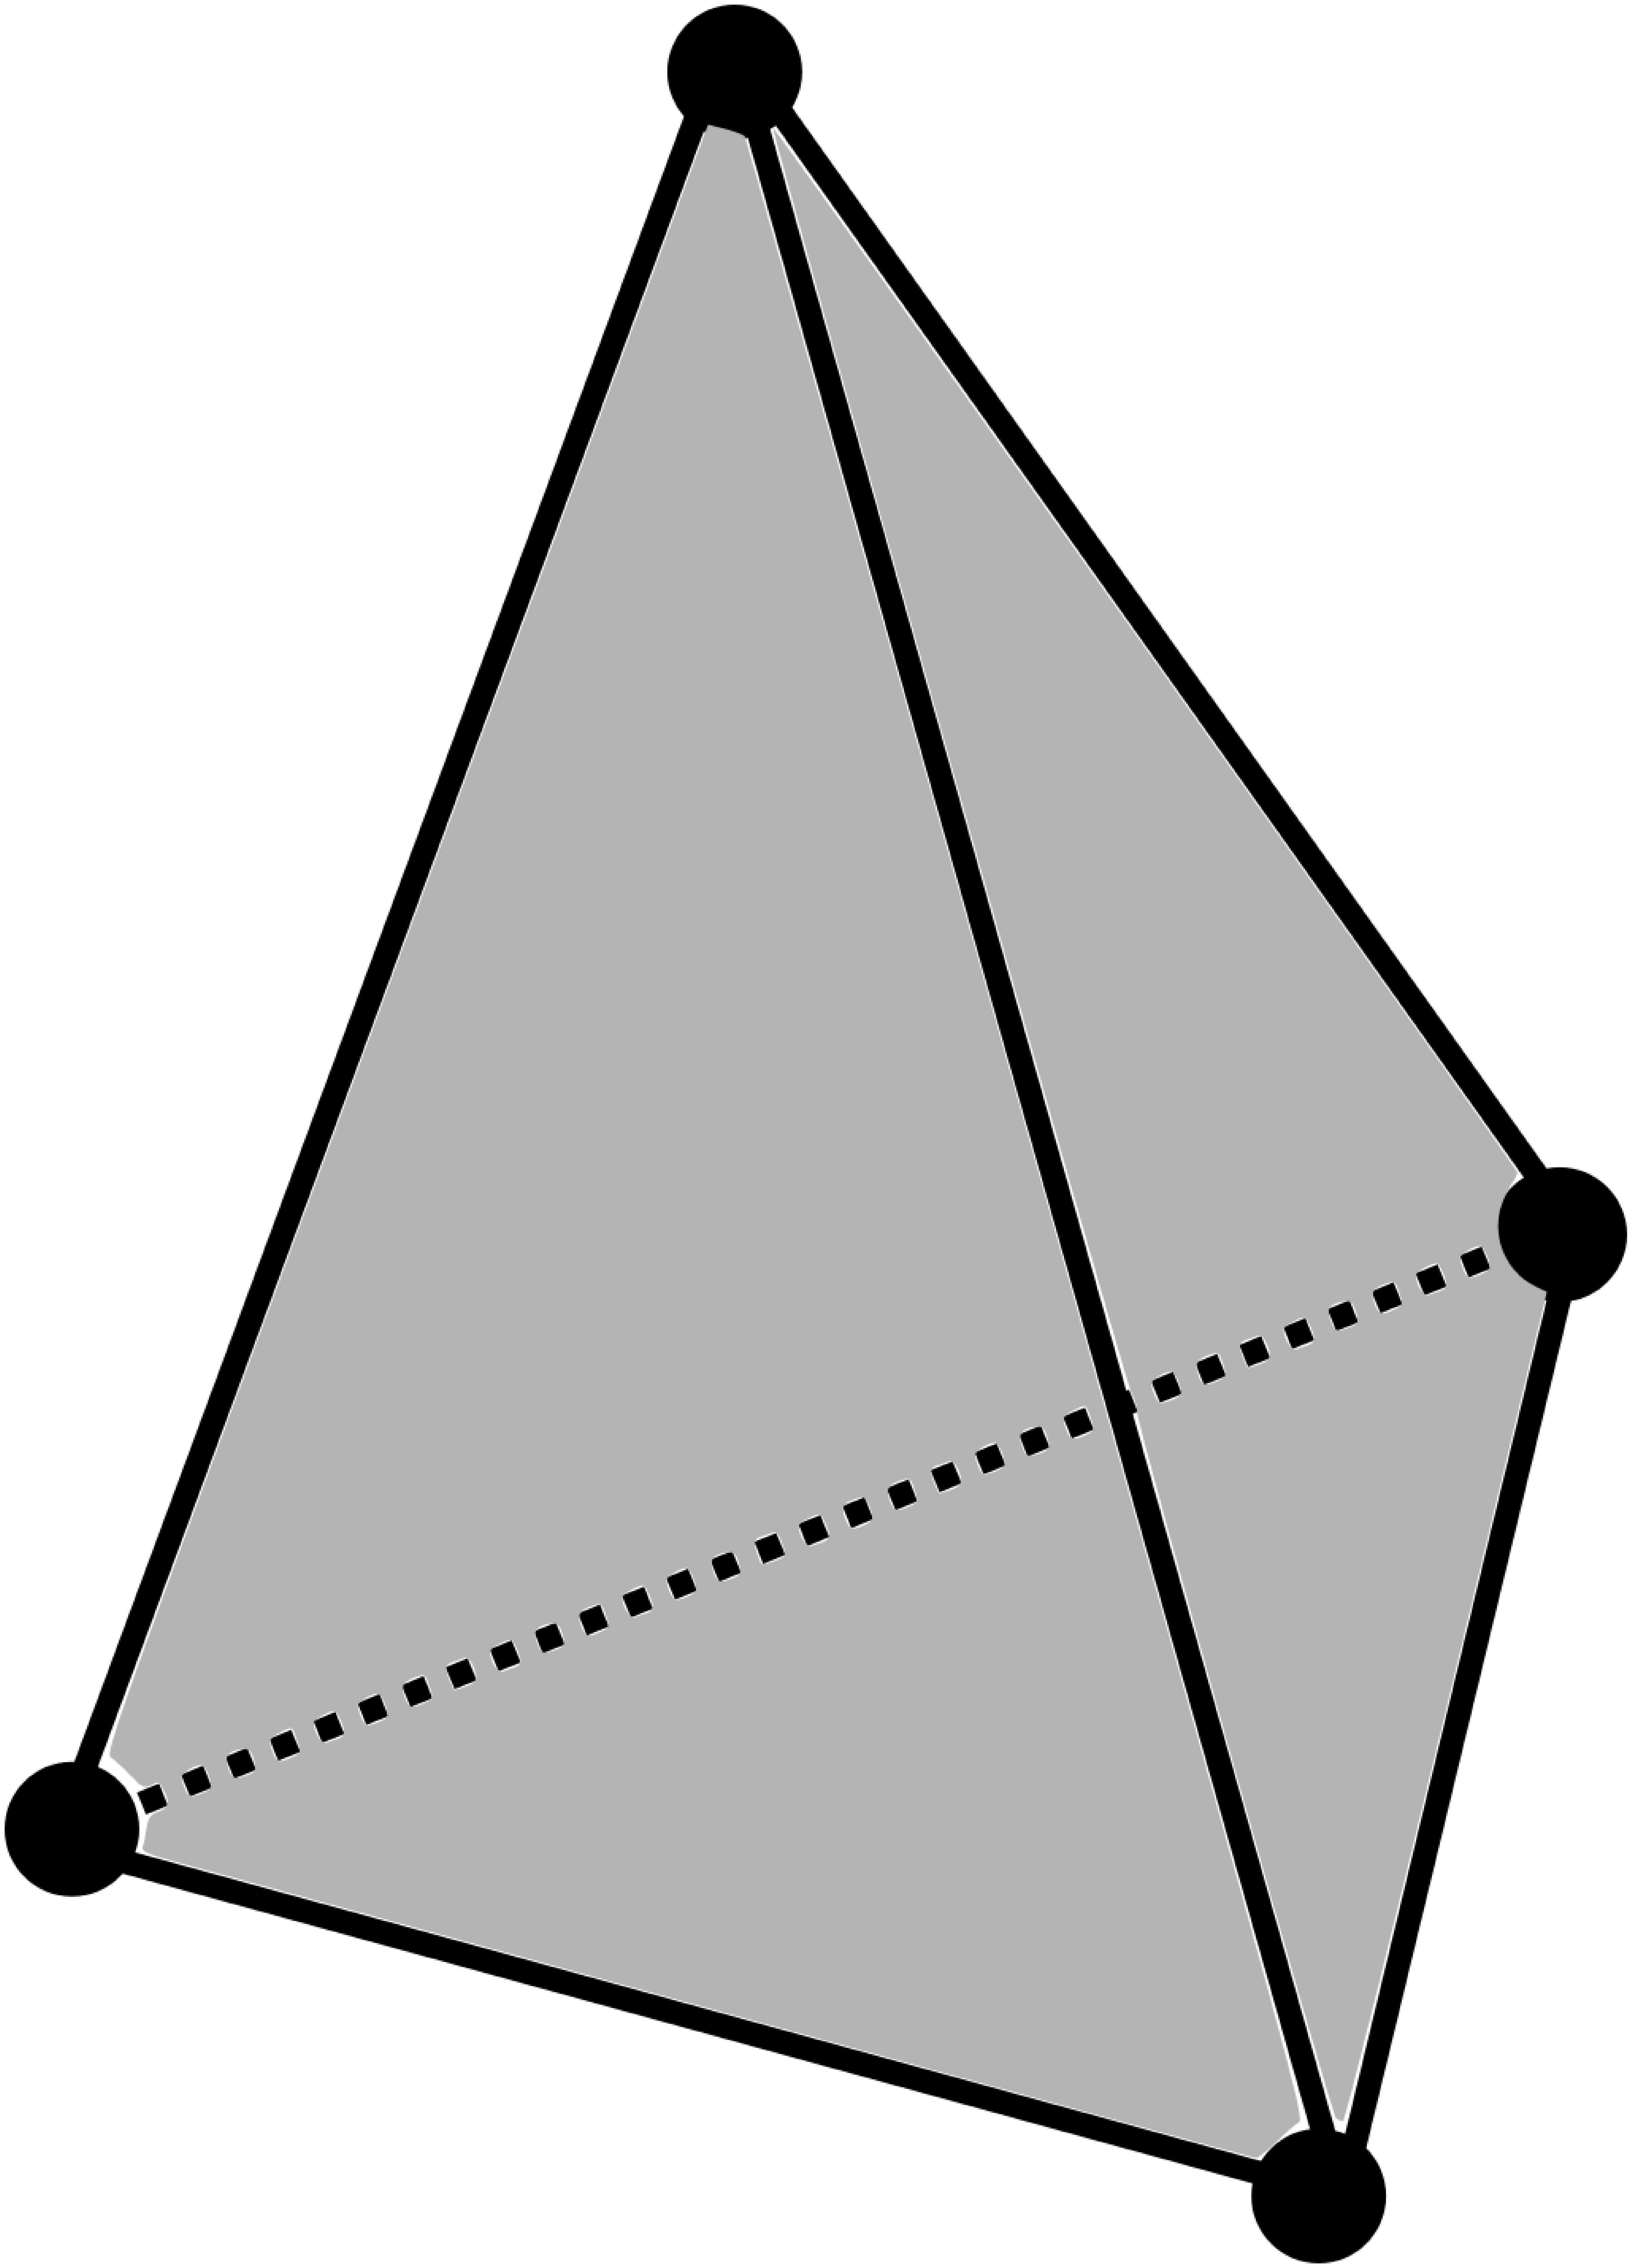
\includegraphics[scale=0.025]{./images/simplex/tet.eps}}}%

    \caption{The simplices of dimension $0, 1, 2$ and $3$.}%
    \label{fig:example}%
\end{figure}

In the definition above the number $k$ is also called the dimension of the simplex. * Analogous to how we mentioned that we will only make use of low dimensional manifolds, here we will only be considering simplices of dimension up to three.*  We will call the simplices of dimension $0, 1, 2 \text{ and } 3$ vertices, edges, triangles and tetrahedron respectively.

A face of a simplex is the convex hull of a non-empty subsets of its points. *Thus the points that define the simplex are its vertices.* To obtain a simplical complex all we have to do is take the union of a number of simplices in the same *ambient dimension* and glue them along common faces without allowing self-intersection. More formally:

\begin{defn} A simplical complex $K$ is a finite collection of simplices such that if $\tau$ is a simplex $K$ then all faces of $\tau$ must be simplicies in $K$. Furthermore the intersection of two simplicies in $K$ is either empty or a common face of both.  \end{defn}


\begin{figure}[h]%
    \centering
    
\includegraphics[center, scale=0.03 ]{./images/simplex/complex.eps}
    \caption{A simplicial comlex}%
    \label{fig:case1.1}%
\end{figure}

We shall obtain the topology of a simplex through embedding it in three-dimensional Euclidean space and consider the subspace topology as a subset. Now that we have formalised the concept of a simplical complex let us see what kind of algebraic invariants we can compute from it.


\subsection{Euler Characteristic}

The first topological invariant of algebraic nature we shall encounter is the Euler Characteristic. It is denoted as $\chi$ and it assigns an integer to simplical complexes through a generalisation of counting \cite{elementary-applied-topology}. The concept was originally defined for polyhedra as a alternating sum of the form $|V| - |E| + |F|$, where $V$ is the set of vertices, $E$ the set of edges and $F$ the set of faces. For example this allowed for the classification of the Platonic solids [].

% @TODO Define CW complexes, simplical complexes may not generalise polyhedra
The Euler Characteristic can be generalized to all spaces that can be decomposed into a finite number of cells. Let us first consider simplical complexes *because they generalise polyhedra*. The natural generalisation of the alternating sum is to continue it indefinitely with the number of 3-cells, then 4-cells, etc., as follows

$$ \chi = k_0 - k_1 + k_2 - ... = \sum_{i}{(-1)^i~k_i}, $$

where all $k_i$ is the number of $i$ dimensional simplicies and $k_i = 0$ for $i$ bigger than some $n \in \mathbb{Z}^+$ and all $k_i$ for $i \le n$ are positive integers.

* Show Examples *

\begin{lem}   The Euler Characteristic is homotopy invariant. \end{lem}

This result allows us to compute the Euler Characteristic of topological spaces which are not simplicial complexes. Let us take for example one of the simplest surfaces - the sphere. We will call any simplicial complex that is homeomorphic to the sphere it's triangulation. The most basic triangulation of the sphere is the tetrahedron. Therefore if we wish to compute the Euler Characteristic of the sphere all we need to do is compute the Euler Characteristic of the tetrahedron. We will use a similar process to compute the contour tree in the next chapter. We will start with an assumption that we have a bounded volume in $\mathbb{R}^2$ and we will triangulate it to enable computation of a topolthe conture tree.

%This results allows to compute in practice $\chi$ of manifolds by considering any of their finite triangulations. As long as there is a homeomorphism between a manifold and triangulation $\chi$ will not change. We will be well advised to pick the triangulations with the least number of simplices to improve computational efficiency. For example the octahedron is a triangulation of a sphere and therefore the Euler Characteristic of the sphere is zero. For further information on this subject we refer the reader to [].
